\documentclass[12pt]{article}
\usepackage{amsmath}
\usepackage{amssymb}
\usepackage{tikz}
\usepackage{pgfplots}
\usepackage{graphicx}
\usepackage{caption}

\title{\textbf{Parabolas}}\\
\author{Tutoring Centre Ferndale\\

\includegraphics[width=4em]{ApS_logo.png}}
\date{}

\begin{document}

\maketitle

\section*{Standard form}
A parabola is the curve made by plotting the graph of a quadratic equation of the form 
\[
y = ax^2 + bx + c
\]
where \(a\), \(b\), and \(c\) are constants.

\begin{center}
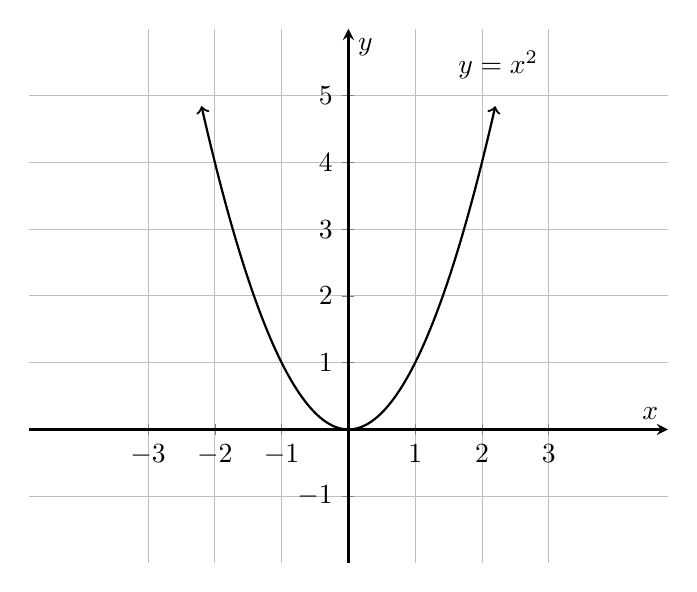
\begin{tikzpicture}
\begin{axis}[width=0.8\textwidth,
    axis line style={<->, thick},
    axis lines = middle,
    xlabel = {$x$},
    ylabel = {$y$},
    domain=-3:6,
    xmin=-4, xmax=4,
    ymin=-2, ymax=6,
    samples=100,
    clip=true,
    ytick={-1,0,1,2,3,4,5},
    xtick={-3,-2,-1,0,1,2,3},
    grid=both,
    grid style={line width=.3pt, draw=gray!50},
    axis equal
]
\addplot [thick, domain=-2.2:2.2,<->] {x^2};
\node at (axis cs:1.5,5.1) [anchor=south west] {$y=x^2$};
\end{axis}
\end{tikzpicture}
\end{center}

\subsection*{Effect of the Leading Coefficient \(a\)}
\begin{itemize}
    \item If \(|a|\) is large, the parabola is narrow.
    \item If \(|a|\) is small, the parabola is wide.
    \item If \(a > 0\), the parabola opens upwards.
    \item If \(a < 0\), the parabola opens downwards.
\end{itemize}

\begin{center}
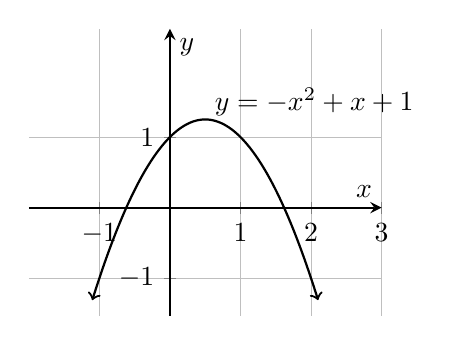
\begin{tikzpicture}
\begin{axis}[width=0.5\textwidth,
    axis line style={<->, thick},
    axis lines = middle,
    xlabel = {$x$},
    ylabel = {$y$},
    domain=-3:6,
    xmin=-2, xmax=3,
    ymin=-1, ymax=2,
    samples=100,
    clip=false,
    ytick={-1,0,1},
    xtick={-1,0,1,2,3},
    grid=both,
    grid style={line width=.3pt, draw=gray!50},
    axis equal
]
\addplot [thick, domain=-1.1:2.1,<->] {-x^2+x+1};
\node at (axis cs:0.5,1.5) [anchor=west] {$y=-x^2+x+1$};
\end{axis}
\end{tikzpicture}
\end{center}

\subsection*{Effect of the Linear Coefficient \(b\)}
\begin{itemize}
\item The coefficient \(b\) shifts the vertex left or right on the $x$-axis, but it is also affected by the value of $a$.
\end{itemize}

\subsection*{Effect of the Constant Term \(c\)}
\begin{itemize}
    \item The coefficient \(c\) moves the entire parabola up or down.
    \item Setting $x$ to 0, the first two terms disappear, leaving only $c$.
    \item The parabola passes through $(0,c)$ so $c$ gives the $y$-intercept.
\end{itemize}

\newpage

\section*{Finding the Roots}
The roots of a quadratic equation are the points where its parabola crosses the $x$-axis. They are the values of \(x\) for which \(y = 0\). Roots are found by various methods of factorizing the quadratic equation, by completing the square, or by using the quadratic formula.

\subsection*{The Discriminant}
The discriminant \(b^2 - 4ac\) shows whether the parabola crosses the x-axis, touches it, or does not cross it.

\begin{itemize}
    \item If \(b^2-4ac > 0\), there are two real roots (the parabola crosses the $x$-axis twice).
    \item If \(b^2-4ac = 0\), there is one real root (the vertex lies on the x-axis).
    \item If \(b^2-4ac < 0\), there are no real roots (the parabola does not cross the x-axis).
\end{itemize}

\subsubsection*{$b^2-4ac > 0$: Parabola with Two Distinct Real Roots\\
(Crosses the $x$-axis twice)}

\begin{center}
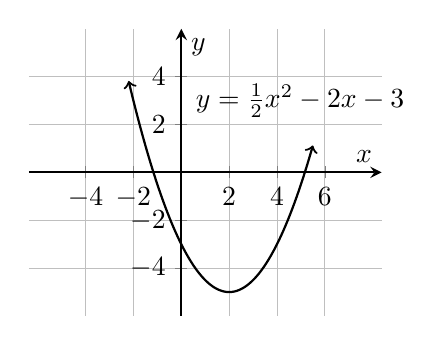
\begin{tikzpicture}
\begin{axis}[width=0.5\textwidth,
    axis line style={<->, thick},
    axis lines = middle,
    xlabel = {$x$},
    ylabel = {$y$},
    domain=-3:6,
    xmin=-4, xmax=6,
    ymin=-6, ymax=6,
    samples=100,
    clip=false,
    ytick={-4,-2,0,2,4},
    xtick={-4,-2,0,2,4,6},
    grid=both,
    grid style={line width=.3pt, draw=gray!50},
    axis equal
]
\addplot [thick, domain=-2.2:5.5,<->]
    {0.5*x^2 - 2*x - 3};
\node at (axis cs:0.2,3) [anchor=west] {$y=\frac{1}{2}x^2 - 2x - 3$};
\end{axis}
\end{tikzpicture}
\end{center}

\subsubsection*{$b^2-4ac=0$: Parabola with One Real Root\\
(Vertex on the $x$-axis) (A perfect square quadratic)}

\begin{center}
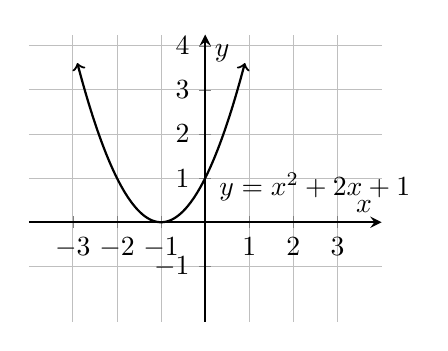
\begin{tikzpicture}
\begin{axis}[width=0.5\textwidth,
    axis line style={<->, thick},
    axis lines = middle,
    xlabel = {$x$},
    ylabel = {$y$},
    domain=-3:6,
    xmin=-4, xmax=4,
    ymin=-2, ymax=4,
    samples=100,
    clip=false,
    ytick={-1,0,1,2,3,4},
    xtick={-3,-2,-1,0,1,2,3},
    grid=both,
    grid style={line width=.3pt, draw=gray!50},
    axis equal
]
\addplot [thick, domain=-2.9:0.9,<->] {x^2+2*x+1};
\node at (axis cs:0.1,0.8) [anchor=west] {$y=x^2+2x+1$};
\end{axis}
\end{tikzpicture}
\end{center}

\subsubsection*{$b^2-4ac<0$: Parabola with No Real Roots\\
(Does not cross the $x$-axis)}

\begin{center}
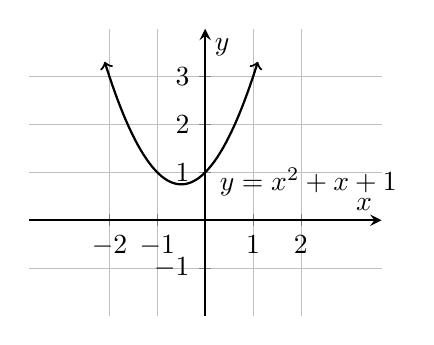
\begin{tikzpicture}
\begin{axis}[width=0.5\textwidth,
    axis line style={<->, thick},
    axis lines = middle,
    xlabel = {$x$},
    ylabel = {$y$},
    domain=-3:6,
    xmin=-3, xmax=3,
    ymin=-2, ymax=4,
    samples=100,
    clip=false,
    ytick={-1,0,1,2,3},
    xtick={-2,-1,0,1,2},
    grid=both,
    grid style={line width=.3pt, draw=gray!50},
    axis equal
]
\addplot [thick, domain=-2.1:1.1,<->] {x^2+x+1};
\node at (axis cs:0.1,0.8) [anchor=west] {$y=x^2+x+1$};
\end{axis}
\end{tikzpicture}
\end{center}

\section*{Vertex Form}
The vertex of the parabola, also called the point of symmetry, is the point where the curve changes direction.\\

The quadratic equation can be written in vertex form:
\[
y = a(x-h)^2 + k
\]
where \((h, k)\) is the vertex of the parabola.\\

\subsection*{Axis of Symmetry}

The $x$-coordinate of the vertex is given by
\[
x_v = -\frac{b}{2a}
\]

The $x$-coordinate of the vertex gives the axis of symmetry of the parabola, which is the line $x=-\frac{b}{2z}$.\\

The $y$-coordinate of the vertex is given by:
\[
y_v = \frac{4ac-b^2}{4a}
\]

\begin{center}
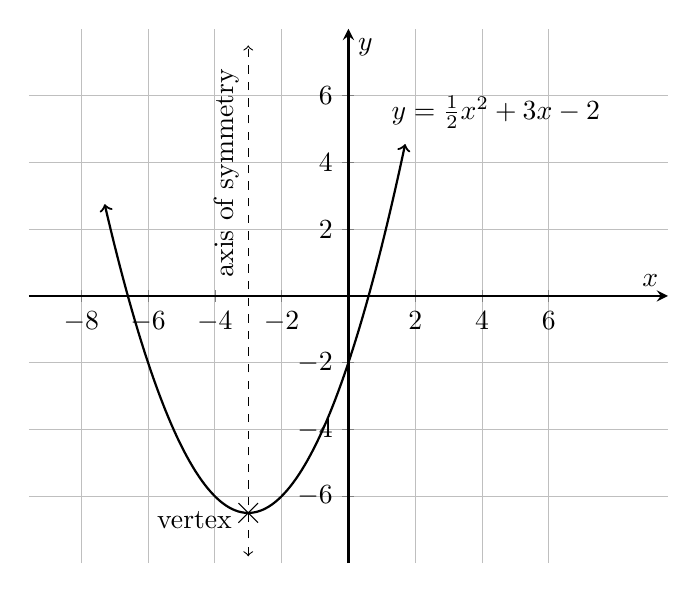
\begin{tikzpicture}
\begin{axis}[width=0.8\textwidth,
    axis line style={<->, thick},
    axis lines = middle,
    xlabel = {$x$},
    ylabel = {$y$},
    domain=-3:6,
    xmin=-8, xmax=8,
    ymin=-8, ymax=8,
    samples=100,
    clip=true,
    ytick={-6,-4,-2,0,2,4,6},
    xtick={-8,-6,-4,-2,0,2,4,6},
    grid=both,
    grid style={line width=.3pt, draw=gray!50},
    axis equal
]
\addplot [thick, domain=-7.3:1.7,<->] {0.5*x^2+3*x-2};
\addplot[mark=x, mark size=5, only marks] coordinates {(-3,-6.5)};
\node at (axis cs:1,5.5) [anchor=west] {$y=\frac{1}{2}x^2+3x-2$};
\draw[dashed,<->] (axis cs:-3,-7.8) -- (axis cs:-3,7.5)
            node[pos=0.75,sloped,above] {axis of symmetry};
\node at (axis cs:-3.2,-6.7) [anchor=east] {vertex};
\end{axis}
\end{tikzpicture}
\end{center}

\newpage

\subsection*{Standard form to Vertex form}
An equation in standard quadratic form is converted to vertex form by completing the square.\\

\textbf{For example,} $y=2x^2+8x+5$ :
\begin{enumerate}
\item Normalize by factoring the first two terms: $y=2(x^2+4x)+5$
\item Complete the square (add and subtract $\frac{b}{2}^2): y=2(x^2+4x+4-4)+5$
\item Perfect Square: $y=2((x+2)^2-4)+5$
\item Distribute the factor of 2: $y=2(x+2)^2-8+5$
\item Vertex form: $y=2(x+2)^2-3$
\end{enumerate}

\subsection*{Vertex form to Standard form}
A quadratic equation in vertex form is changed to standard form by multiplying it out and rearranging.\\

\textbf{For example,} $y=2(x+2)^2-3$ :
\begin{enumerate}
\item $y=2(x+2)^2-3 \implies y=2(x+2)(x+2)-3$
\item FOIL: $y=2(x^2+2x+2x+4)-3$
\item Distribute the factor of 2: $y=(2x^2+4x+4x+8)-3$
\item Combine like terms: $y=2x^2+8x+5$ (Standard form.)
\end{enumerate}

\newpage

\section*{Drawing a Parabola from its equation}

Given a quadratic equation, five point of the parabola can be plotted and the curve sketched.

\begin{itemize}
    \item If $a$ is positive the parabola opens upwards.
    \item The roots of the parabola are given by the quadratic formula.
    \item The coordinates of the vertex are $(-\frac{b}{2a},\frac{4ac-b^2}{4a})$.
    \item The $y$-intercept, where $x=0$, is given by $c$.
    \item The symmetry point to the $y$-intercept is $(2h, c)$.
    \item More points can be plotted by calculating values of $y$ for given values of $x$. Use the axis of symmetry as the middle $x$-value and find $x$-values on either side.
\end{itemize}

\textbf{For example,} to graph $y=2x^2+4x-1$:

\begin{itemize}
    \item $a$ is positive so the parabola opens upwards.
    \item From the quadratic formula,\\the roots are $\frac{-2+\sqrt{6}}{2}$ and $\frac{-2-\sqrt{6}}{2} \ (\approx 0.225 \ \& -2.225$.)
    \item The $x$-coordinate of the vertex, which also gives the axis of symmetry, is $x=-\frac{b}{2a}=-\frac{4}{2\cdot2}=-1$.
    \item The $y$-coordinate of the vertex, by substituting $x=-1$ into the\\equation, is $y=2(-1)^2+4(-1)-1=2-4-1=-3$.
    \item The $y$-intercept is given by $c=-1$.
    \item The symmetry point to the $y$-intercept is $(2h, c) = (-2,-1)$.
    \item Plotting a couple of extra points either side of the axis of symmetry:\\
    For $x=-2.5, y=2(-2.5)^2+4(-2.5)-1=1.5$.\\
    For $x= 0.5, y=2(0.5)^2+4(0.5)-1==1.5$.
    \item That's 7 points to plot which makes it easy to draw the curve through them.
\end{itemize}

\begin{center}
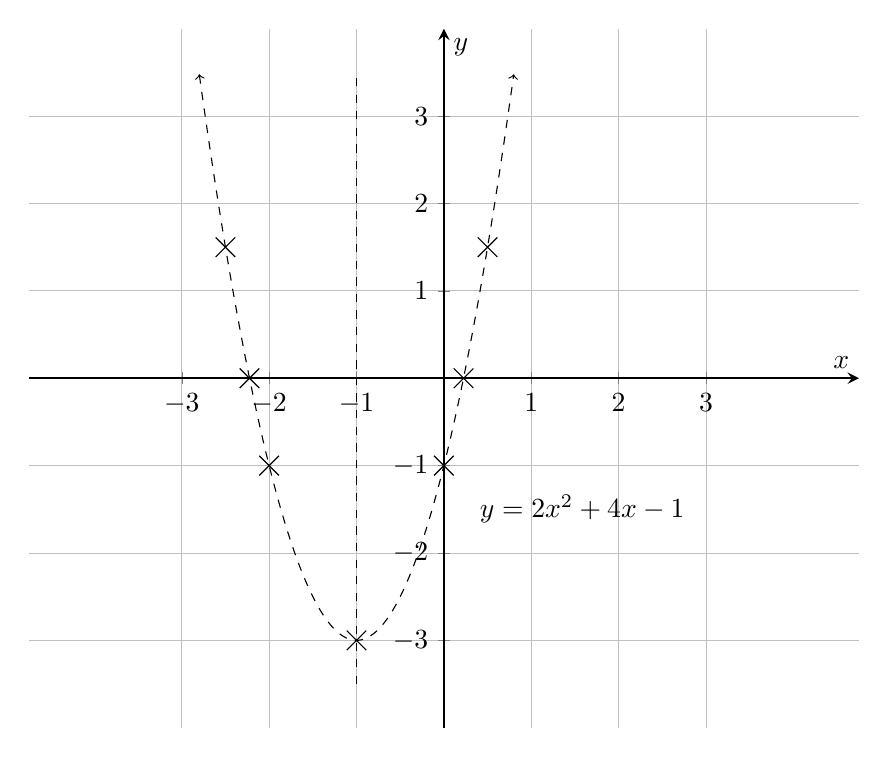
\begin{tikzpicture}
\begin{axis}[width=\textwidth,
    axis line style={<->, thick},
    axis lines = middle,
    xlabel = {$x$},
    ylabel = {$y$},
    domain=-3:6,
    xmin=-3, xmax=3,
    ymin=-4, ymax=4,
    samples=100,
    clip=true,
    ytick={-3,-2,-1,0,1,2,3},
    xtick={-3,-2,-1,0,1,2,3},
    grid=both,
    grid style={line width=.3pt, draw=gray!50},
    axis equal
]
\addplot [thin, dashed, domain=-2.8:0.8,<->] {2*x^2+4*x-1};
\node at (axis cs:0.3,-1.5) [anchor=west] {$y=2x^2+4x-1$};
\addplot[mark=x, mark size=5, only marks] coordinates {(-2.225,0)(0.225,0)(-1,-3)(0,-1)(-2,-1)(-2.5,1.5)(0.5,1.5)};
\draw [dashed] (-1,-3.5) -- (-1,3.5);
\end{axis}
\end{tikzpicture}
\end{center}

\section*{Solving quadratic equations graphically}
Instead of doing the maths to factorize a quadratic equation or calculate its roots with the quadratic formula, it is sometimes more practical to plot the parabolic curve of the equation and read the solution from the graph.\\

For example, to find the roots and vertex of $y=x^2-2x$:\\

The axis of symmetry is $x=-\frac{b}{2a}=-\frac{-2}{2}=1$, so calculating some points either side of that:
\begin{table}[h]
    \centering
    \begin{tabular}{c|c|c|c|c|c}
         x & -1 & 0 &  1 & 2 & 3 \\\hline
         y &  3 & 0 & -1 & 0 & 3 
    \end{tabular}
    \caption*{$y=x^2-2x$}
\end{table}

Plotting these coordinates and drawing a curve between them:

\begin{center}
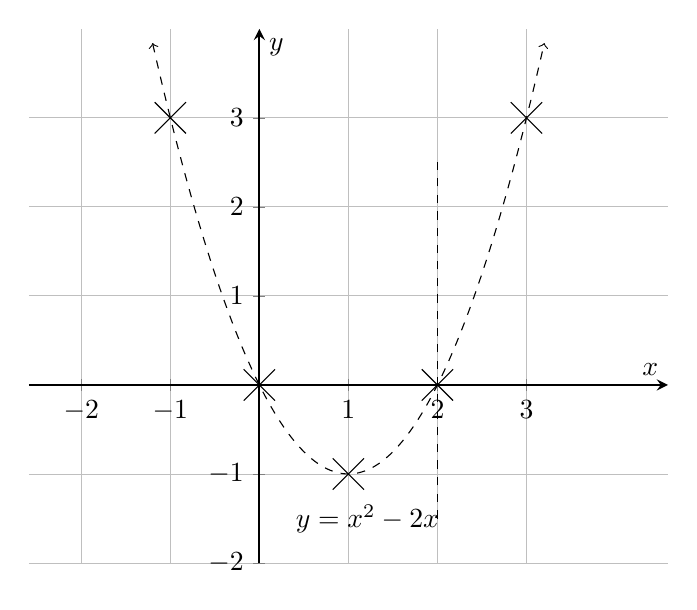
\begin{tikzpicture}
\begin{axis}[width=0.8\textwidth,
    axis line style={<->, thick},
    axis lines = middle,
    xlabel = {$x$},
    ylabel = {$y$},
    domain=-3:6,
    xmin=-2, xmax=4,
    ymin=-2, ymax=4,
    samples=100,
    clip=true,
    ytick={-2,-1,0,1,2,3},
    xtick={-2,-1,0,1,2,3},
    grid=both,
    grid style={line width=.3pt, draw=gray!50},
    axis equal
]
\addplot [thin, dashed, domain=-1.2:3.2,<->] {x^2-2*x};
\node at (axis cs:0.3,-1.5) [anchor=west] {$y=x^2-2x$};
\addplot[mark=x, mark size=8, only marks] coordinates {(-1,3)(0,0)(1,-1)(2,0)(3,3)};
\draw [dashed] (2,-1.5) -- (2,2.5);
\end{axis}
\end{tikzpicture}
\end{center}

The roots can be seen at $(0,0)$ and $(2,0)$, and the vertex is at $(1,-1)$.

\section*{Finding a quadratic equation\\given its roots and vertex}

Given an observed parabola, such as the path of a thrown object, it is possible to work out its equation.\\

Say an object was fired into the air, reached a height of 300 metres, and landed 200 metres away. That gives us 3 coordinates: The roots are at (0,0) and 200,0). The axis of symmetry is halfway between the starting and ending points, at 100 metres, and the vertex is at (100, 300).\\

Substituting the vertex (100, 00) into the vertex form of a quadratic equation, we get $y=a(x-100)^2+300$.\\

\newpage

To find $a$, substitute either of the roots into this. Using (0,0): $0=a(0-100)^2+300 \implies a=-\frac{3}{100}$.\\

Substituting $a=-\frac{3}{100}$ back into the equation: $y=-\frac{3}{100}(x-100)^2+300$.\\

Rearranging this to get the equation from vertex form into standard form: $y=-\frac{3}{100}x^2+6x$.\\

\begin{center}
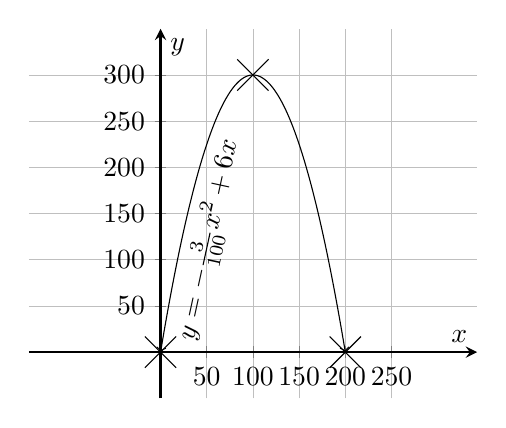
\begin{tikzpicture}
\begin{axis}[width=0.6\textwidth,
    axis line style={<->, thick},
    axis lines = middle,
    xlabel = {$x$},
    ylabel = {$y$},
    domain=-50:250,
    xmin=-50, xmax=250,
    ymin=-50, ymax=350,
    samples=100,
    clip=false,
    ytick={0,50,100,150,200,250,300},
    xtick={0,50,100,150,200,250},
    grid=both,
    grid style={line width=.3pt, draw=gray!50},
    axis equal
]
\addplot [->,thin, domain=0:200, <->] {-0.03*x^2+6*x} node[pos=0.2,sloped,below]{$y=-\frac{3}{100}x^2+6x$};
\addplot[mark=x, mark size=8, only marks] coordinates {(0,0)(100,300)(200,0)};
\end{axis}
\end{tikzpicture}
\end{center}

Any point along the curve can now be calculated.\\

\textbf{Another method of finding the equation given roots and vertex:}\\

Given the roots (1,0),(-5,0) and the vertex at (-2,-9), form an equation from the roots using the null factor law:
\begin{table}[h]
    \centering
    \begin{tabular}{r|r}
         $ x=1 $ & $   x=-5 $  \\
         x-1=0   & $ x+5=0$ \\
\end{tabular}
\end{table}

$(x-1)(x+5)=0 \implies x^2+4x-5=0$\\

\noindent
Other parabolas can share these roots\\so verify by substituting in the vertex $(-2,-9)$:
\begin{align*}
-2^2+4(-2)-5&=-9\\
-9&=-9 \ \checkmark
\end{align*}

\section*{Finding a quadratic equation\\given the vertex and a point on the parabola}

\begin{itemize}
\item Vertex: $(2,3) \ [h=2,k=-3]$
\item A point on the curve: $(5,6)$
\end{itemize}

The quadratic equation in vertex form: $y=a(x-2)^2-3$

Multiply out to get standard form: 
\begin{align*}
y&=a(x-2)^2-3\\
y&=a(x-2)(x-2)-3\\
y&=ax^2-2x-2x+4-3\\
y&=ax^2-4x+1
\end{align*}

Substitute in the given $(x,y)$ coordinate:
\begin{align*}
6&=a\cdot5^2-4\cdot5+1\\
6&=a\cdot25-20+1\\
6&=a\cdot25\\
a&=1
\end{align*}

The equation is $y=x^2-4x+1$\\

Graphing this:

\begin{itemize}
\item Given vertex: $(2,3)$
\item Given point: $5,6$
\item Roots: $x = \frac{-(-4)\pm\sqrt{-4^2-4\cdot1\cdot1}}{2\cdot1} = \frac{4\pm\sqrt{12}}{2} \approx 3.73 \ \& 0.27$
\item $y$-intercept $= c = 1$
\item Symmetrically opposite point to y-intercept: $(2h,c) = (4,1)$
\end{itemize}

\begin{center}
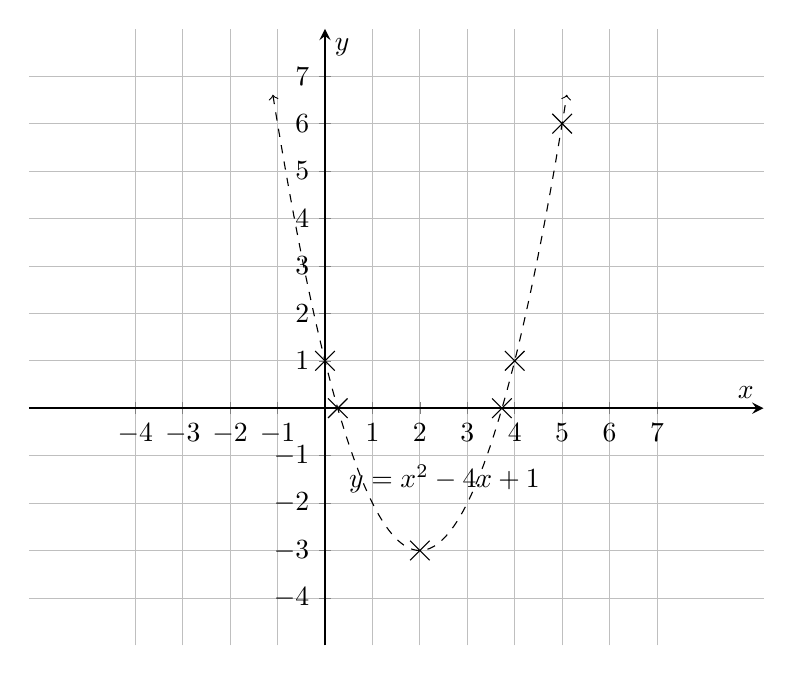
\begin{tikzpicture}
\begin{axis}[width=0.9\textwidth,
    axis line style={<->, thick},
    axis lines = middle,
    xlabel = {$x$},
    ylabel = {$y$},
    domain=-3:6,
    xmin=-5, xmax=8,
    ymin=-5, ymax=8,
    samples=100,
    clip=true,
    ytick={-4,-3,-2,-1,0,1,2,3,4,5,6,7},
    xtick={-4,-3,-2,-1,0,1,2,3,4,5,6,7},
    grid=both,
    grid style={line width=.3pt, draw=gray!50},
    axis equal
]
\addplot [thin, dashed, domain=-1.1:5.1,<->] {x^2-4*x+1};
\node at (axis cs:0.3,-1.5) [anchor=west] {$y=x^2-4x+1$};
\addplot[mark=x, mark size=5, only marks] coordinates {(2,-3)(5,6)(3.73,0)(0.27,0)(0,1)(4,1)};
\end{axis}
\end{tikzpicture}
\end{center}

\section*{Finding points of intersection }

\subsection*{Intersection of Two Lines}
At the point where two lines intersect, that coordinate satisfies both linear equations simultaneously.\\

Given two lines:
\[
y = m_1x + c_1
\]
\[
y = m_2x + c_2
\]
To find their intersection, set the two equations equal to each other:
\[
m_1x + c_1 = m_2x + c_2
\]

Solve for $x$, and then substitute \(x\) back into either equation to find \(y\).\\

\newpage

\textbf{For example,}\\

Find the intersection of the lines \( y = 2x + 1 \) and \( y = -x + 4 \).
\[
\begin{aligned}
2x + 1 &= -x + 4 \\
3x &= 3 \\
x &= 1 \\
y &= 2(1) + 1 = 3
\end{aligned}
\]
The intersection point is \( (1, 3) \):

\begin{center}
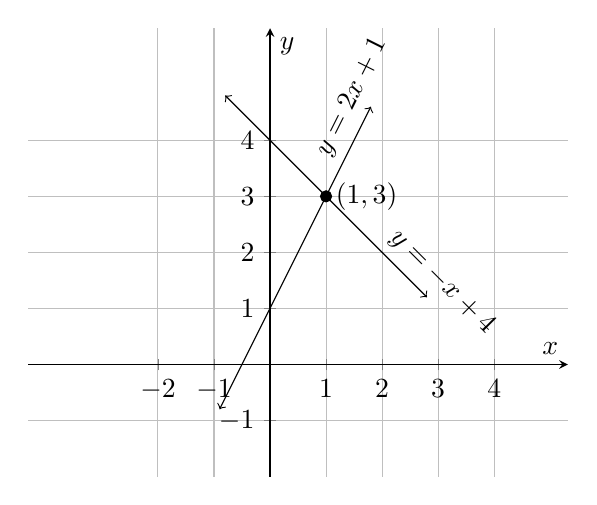
\begin{tikzpicture}
    \begin{axis}[
        axis lines = middle,
        xlabel = \(x\),
        ylabel = \(y\),
        ymin=-2, ymax=6, 
        xmin=-2, xmax=3,
        ytick={-1,0,1,2,3,4},
        xtick={-2,-1,0,1,2,3,4},
        grid = both,
        axis equal
    ]
    \addplot [thin, domain=-0.9:1.8,<->] {2*x+1}    node[pos=1,sloped, above]{$y=2x+1$};
    \addplot [thin, domain=-0.8:2.8,<->] {-x+4}    node[pos=1,sloped, above]{$y=-x+4$};
    \addplot[mark=*, only marks] coordinates {(1,3)} node[right]{$(1,3)$};
    \end{axis}
\end{tikzpicture}
\end{center}

\subsection*{Intersection of a Line and a Parabola}
The intersection points of a line and a parabola occur where the coordinates satisfy both equations. That point is found by substituting the linear equation into the quadratic equation and solving the resulting quadratic equation.\\

Given a line \( y = mx + c \) and a parabola \( y = ax^2 + bx + d \), substitute the linear equation into the quadratic:
\[
mx + c = ax^2 + bx + d
\]
Rearrange to form a quadratic equation:
\[
ax^2 + (b-m)x + (d-c) = 0
\]
Solve this quadratic equation for \(x\). Then, substitute the solutions back into the linear equation to find the corresponding \(y\) values.\\

\textbf{For example,}\\

Find the intersection of the line \( y = 2x + 1 \) and the parabola \( y = x^2 + x - 2 \):
\[
\begin{aligned}
2x + 1 &= x^2 + x - 2 \\
0 &= x^2 - x - 3 \\
x &= \frac{1 \pm \sqrt{13}}{2} \ \approx 2.30 \ \& -1.30
\end{aligned}
\]

Substitute these into the line equation to find the corresponding \(y\) values:

$$y = 2(\frac{1\pm\sqrt{13}}{2})+1 \ \approx5.61 \ \& -1.61$$

So the points of intersection are $\approx(2.30,5.61)$ and $\approx(-1.30,-1.61).$
\begin{center}
\begin{tikzpicture}
    \begin{axis}[width=\textwidth,
        axis lines = middle,
        xlabel = \(x\),
        ylabel = \(y\),
        ymin=-3, ymax=8, 
        xmin=-3, xmax=3,
        xtick={-2,-1,0,1,2,3},
        ytick={-2,-1,0,1,2,3,4,5,6,7},
        grid = both,
        axis equal
        ]
    \addplot[<->,domain=-2.5:2.6,thick]{x^2 + x - 2}
    node[pos=0.6,sloped,above]{$y=x^2+x-2$};
    \addplot[<->,domain=-1.9:3.2, thick]{2*x + 1}
    node[pos=0.6,sloped,above]{$y=2x+1$};
    \addplot[mark=*, size=20, only marks]
    coordinates {(2.30,5.61) (-1.30,-1.61)};
    \draw[thin,dashed](axis cs:2.30,5.61)
     node[anchor=west]{$\approx(2.3,5.6)$} -- (axis cs:2.30,0);
    \draw[thin,dashed](axis cs:-1.30,0) -- (axis cs:-1.30,-1.61) node[anchor=east]{$\approx(-1.3,-1.6)$};
    \end{axis}
\end{tikzpicture}
\end{center}

\section*{Solving a quadratic equation by adding a line}

Given any parabola formed by the equation $y=ax^2+bx+c$,\\any quadratic equation $Ax^2+Bx+C=0$ can be solved by drawing a straight line.\\

\noindent
Given:
$$Ax^2+Bx+C=0$$
Divide by A and multiply by a:
$$ax^2+\frac{aB}{A}x+\frac{aC}{A}=0$$
Isolate $ax^2$:
$$ax^2=-\frac{aB}{A}x-\frac{aC}{A}$$
Substitute:
$$ax^2+bx+c=-\frac{aB}{A}x-\frac{aC}{A}+bx+c$$
Factorize into standard linear form:
$$ax^2+bx+c=(b-\frac{aB}{A})x+(c-\frac{aC}{A})$$
The intersection of $y=ax^2+bx+c$ and $y=(b-\frac{aB}{A})x+(c-\frac{aC}{A})$ then solves $y=Ax^2+Bx+C=0$.\\

A graphical solution such as this can be a simpler method when an exact solution is not required.\\

\newpage

\textbf{For example,} Using $y=x^2-2x-4$ to solve $0=2x^2-3x-6$:\\

You could do:\\

Set the equations equal:

$$x^2-2x-4=-\frac{1}{2}x-1$$

Move all terms to one side:

$$2(x^2-2x-4)=2(-\frac{1}{2}x-1)$$
$$2x^2-4x-8=-x-2$$
$$2x^2-4x-8+x+2=0$$
$$2x^2-3x-6=0$$

Use the quadratic formula to find the roots:

$$x=\frac{3\pm\sqrt{57}}{4} \approx 2.64 \ \& -1.14$$

\newpage

But an easier solution could be to draw the parabola and to find the equation of the line to draw across it:

$$y=(b-\frac{aB}{A})x+(c-\frac{aC}{A})$$
$$y=(-2-\frac{1\cdot-3}{2})x+(-4-\frac{1\cdot-6}{2})$$
$$y=(-2+\frac{3}{2})x+(-4+3)$$
$$y=-\frac{1}{2}x-1$$

Plotting these curves and reading off the roots:

\begin{center}
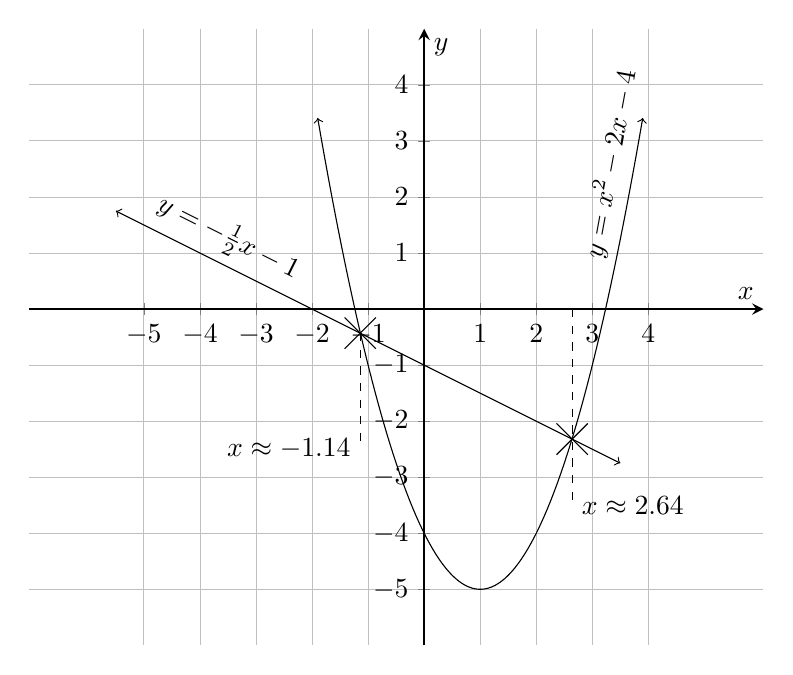
\begin{tikzpicture}
\begin{axis}[width=0.9\textwidth,
    axis line style={<->, thick},
    axis lines = middle,
    xlabel = {$x$},
    ylabel = {$y$},
    domain=-50:250,
    xmin=-5, xmax=4,
    ymin=-6, ymax=5,
    samples=100,
    clip=false,
    ytick={-5,-4,-3,-2,-1,0,1,2,3,4},
    xtick={-5,-4,-3,-2,-1,0,1,2,3,4},
    grid=both,
    grid style={line width=.3pt, draw=gray!50},
    axis equal
]
\addplot [thin, domain=-5.5:3.5, <->] {-0.5*x-1} node[pos=0.2,sloped,above] {$y=-\frac{1}{2}x-1$};
\addplot [thin, domain=-1.9:3.9, <->] {x^2-2*x-4} node[pos=0.95,sloped,above] {$y=x^2-2x-4$};
\draw[thin,dashed] (axis cs:-1.14,-0.43) -- (axis cs:-1.14,-2.5) node[anchor=east]{$x\approx-1.14$};
\draw[thin,dashed] (axis cs:2.64,0) -- (axis cs:2.64,-3.5) node[anchor=west]{$x\approx2.64$};
\addplot[mark=x, mark size=8, only marks] coordinates {(2.64,-2.32)(-1.14,-0.43)};
\end{axis}
\end{tikzpicture}
\end{center}

\newpage

\section*{Using $y=x^2$ to solve a quadratic equation}

In the same way that adding a line can be a simple way to solve a quadratic equation, the parabola $y=x^2$ can be used to solve quadratic equations.\\

\textbf{For example,} Using $y=x^2$ to solve $3x^2-6x-4=0$:

$$3x^2-6x-4=0$$
$$x^2-2x-\frac{4}{3}=0$$
$$x^2=2x+\frac{4}{3}$$

So plot $y=2x+\frac{4}{3}$ and $y=x^2$:
\begin{center}
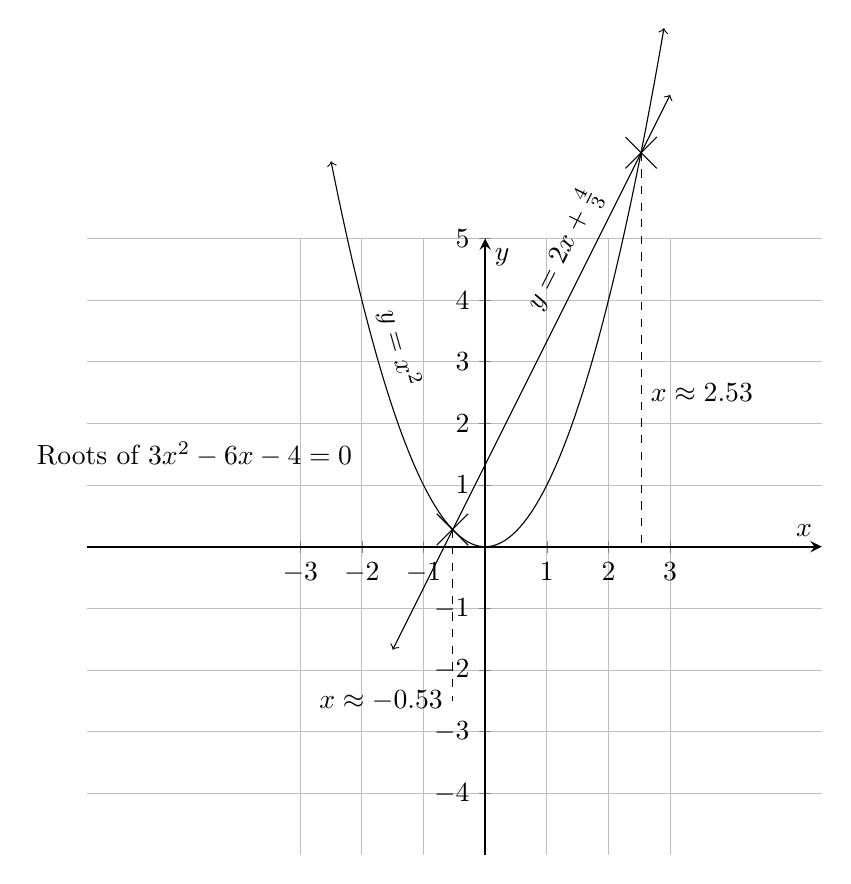
\begin{tikzpicture}
\begin{axis}[width=0.9\textwidth,
    axis line style={<->, thick},
    axis lines = middle,
    xlabel = {$x$},
    ylabel = {$y$},
    domain=-50:250,
    xmin=-5, xmax=4,
    ymin=-5, ymax=5,
    samples=100,
    clip=false,
    ytick={-4,-3,-2,-1,0,1,2,3,4,5,6},
    xtick={-3,-2,-1,0,1,2,3},
    grid=both,
    grid style={line width=.3pt, draw=gray!50},
    axis equal
]
\addplot [thin, domain=-2.5:2.9, <->] {x^2} node[pos=0.2,sloped,above] {$y=x^2$};
\addplot [thin, domain=-1.5:3, <->] {2*x+1.33} node[pos=0.7,sloped,above] {$y=2x+\frac{4}{3}$};
\draw[thin,dashed] (axis cs:-0.53,0.28) -- (axis cs:-0.53,-2.5) node[anchor=east]{$x\approx-0.53$};
\draw[thin,dashed] (axis cs:2.53,6.39) -- (axis cs:2.53,2.5) node[anchor=west]{$x\approx2.53$} -- (axis cs:2.53,0);
\addplot[mark=x, mark size=8, only marks] coordinates {(2.53,6.39)(-0.53,0.28)};
\node[anchor=east] at (axis cs:-2,1.5) {Roots of $3x^2-6x-4=0$};

\end{axis}
\end{tikzpicture}
\end{center}

\end{document}
